\documentclass[11pt,t]{beamer}
\hypersetup{pdfencoding=auto}
%\usefonttheme{professionalfonts}
\usefonttheme[onlymath]{serif}

\usetheme{Berkeley}

\usepackage{xcolor}
\usepackage{amssymb,amsmath,graphicx}
\usepackage{kotex}
\usepackage{multimedia}
\usepackage{setspace}
\usepackage{multicol}
\usepackage{verbatim} %use 
\usepackage{ragged2e}
\addtobeamertemplate{block begin}{}{\justifying}

%% Color Setting %%
\definecolor{Grey}{rgb}{0.6,0.6,0.6}
\definecolor{GSHSred}{RGB}{105,0,0}
\definecolor{GSHSRED}{RGB}{80,0,0}
\definecolor{gshsred}{RGB}{240,210,210}
\setbeamercolor{title}{bg=white,fg=GSHSred}
\setbeamercolor{author}{fg=GSHSred}
\setbeamercolor{institute}{fg=GSHSred}
\setbeamercolor{date}{fg=GSHSred}
\setbeamercolor{logo}{bg=GSHSred}
\setbeamercolor{sidebar}{bg=GSHSred}
\setbeamercolor{frametitle}{bg=white,fg=GSHSred}
\setbeamercolor{section in sidebar}{use=sidebar,bg=white,fg=sidebar.bg}
\setbeamercolor{subsection in sidebar}{parent=section in sidebar}
\setbeamercolor{subsubsection in sidebar}{parent=subsection in sidebar}
\setbeamercolor{item}{fg=GSHSred}
\setbeamercolor{block title}{bg=GSHSRED,fg=white}
\setbeamercolor{block body}{bg=gshsred,fg=black}

%% Frametitle Setting %%
\setbeamerfont{frametitle}{series=\bfseries}
\setbeamertemplate{frametitle}
{ \vspace*{-10mm}
  \leavevmode
  \hspace*{3pt}
  \begin{beamercolorbox}[wd=\paperwidth,ht=1ex,dp=1ex]{frametitle}
    \hspace*{7pt}\underline{\makebox[0.6\paperwidth][l]{
    \Large{\insertframetitle}}}
  \end{beamercolorbox}
}

\makeatletter
\setlength{\beamer@headheight}{0cm}
\makeatother

\logo{
\includegraphics[width=8mm]{./logo/gshslogo.png}}

\makeatletter
\setbeamertemplate{headline}{}

\defbeamertemplate*{sidebar \beamer@sidebarside}{mysidebar theme}
{
	\beamer@tempdim=\beamer@sidebarwidth%
	\advance\beamer@tempdim by -6pt%
	{%
		\begin{beamercolorbox}[wd=\beamer@sidebarwidth, ht=\beamer@sidebarwidth]{logo}
			\begin{minipage}[b][\beamer@sidebarwidth][c]{\beamer@sidebarwidth}  
				\centering%
				\insertlogo%
			\end{minipage}
		\end{beamercolorbox}
		\vskip-.8\beamer@sidebarwidth%
		\usebeamerfont{title in sidebar}%
		\vskip1.5em%
		\hskip3pt%
		\usebeamercolor[fg]{title in sidebar}%
		\insertshorttitle[width=\beamer@tempdim,center,respectlinebreaks]\par%
		\vskip1.25em%
	}%
	{%
		\hskip3pt%
		\usebeamercolor[fg]{author in sidebar}%
		\usebeamerfont{author in sidebar}%
		\insertshortauthor[width=\beamer@tempdim,center,respectlinebreaks]\par%
		\vskip1.25em%
	}%
	\insertverticalnavigation{\beamer@sidebarwidth}%
	\vfill
	\ifx\beamer@sidebarside\beamer@lefttext%
	\else%
	\usebeamercolor{normal text}%
	\llap{\usebeamertemplate***{navigation symbols}\hskip0.1cm}%
	\vskip2pt%
	\fi%
}%
\makeatother
             
%% Title Page Setting %%
%\setbeamerfont{title}{series=\bfseries}
\setbeamertemplate{title page}{
  %% Background Logo
  \begin{picture}(0,0)%
    \setlength{\unitlength}{1cm}% default
    \protect\put(0,0){%
    \begin{picture}(6,6)(4,10)%
    %%%%%%%%%%%%%%%%%%%%%%%%%%%%%%%%%%%%%%%%%%%%%
      %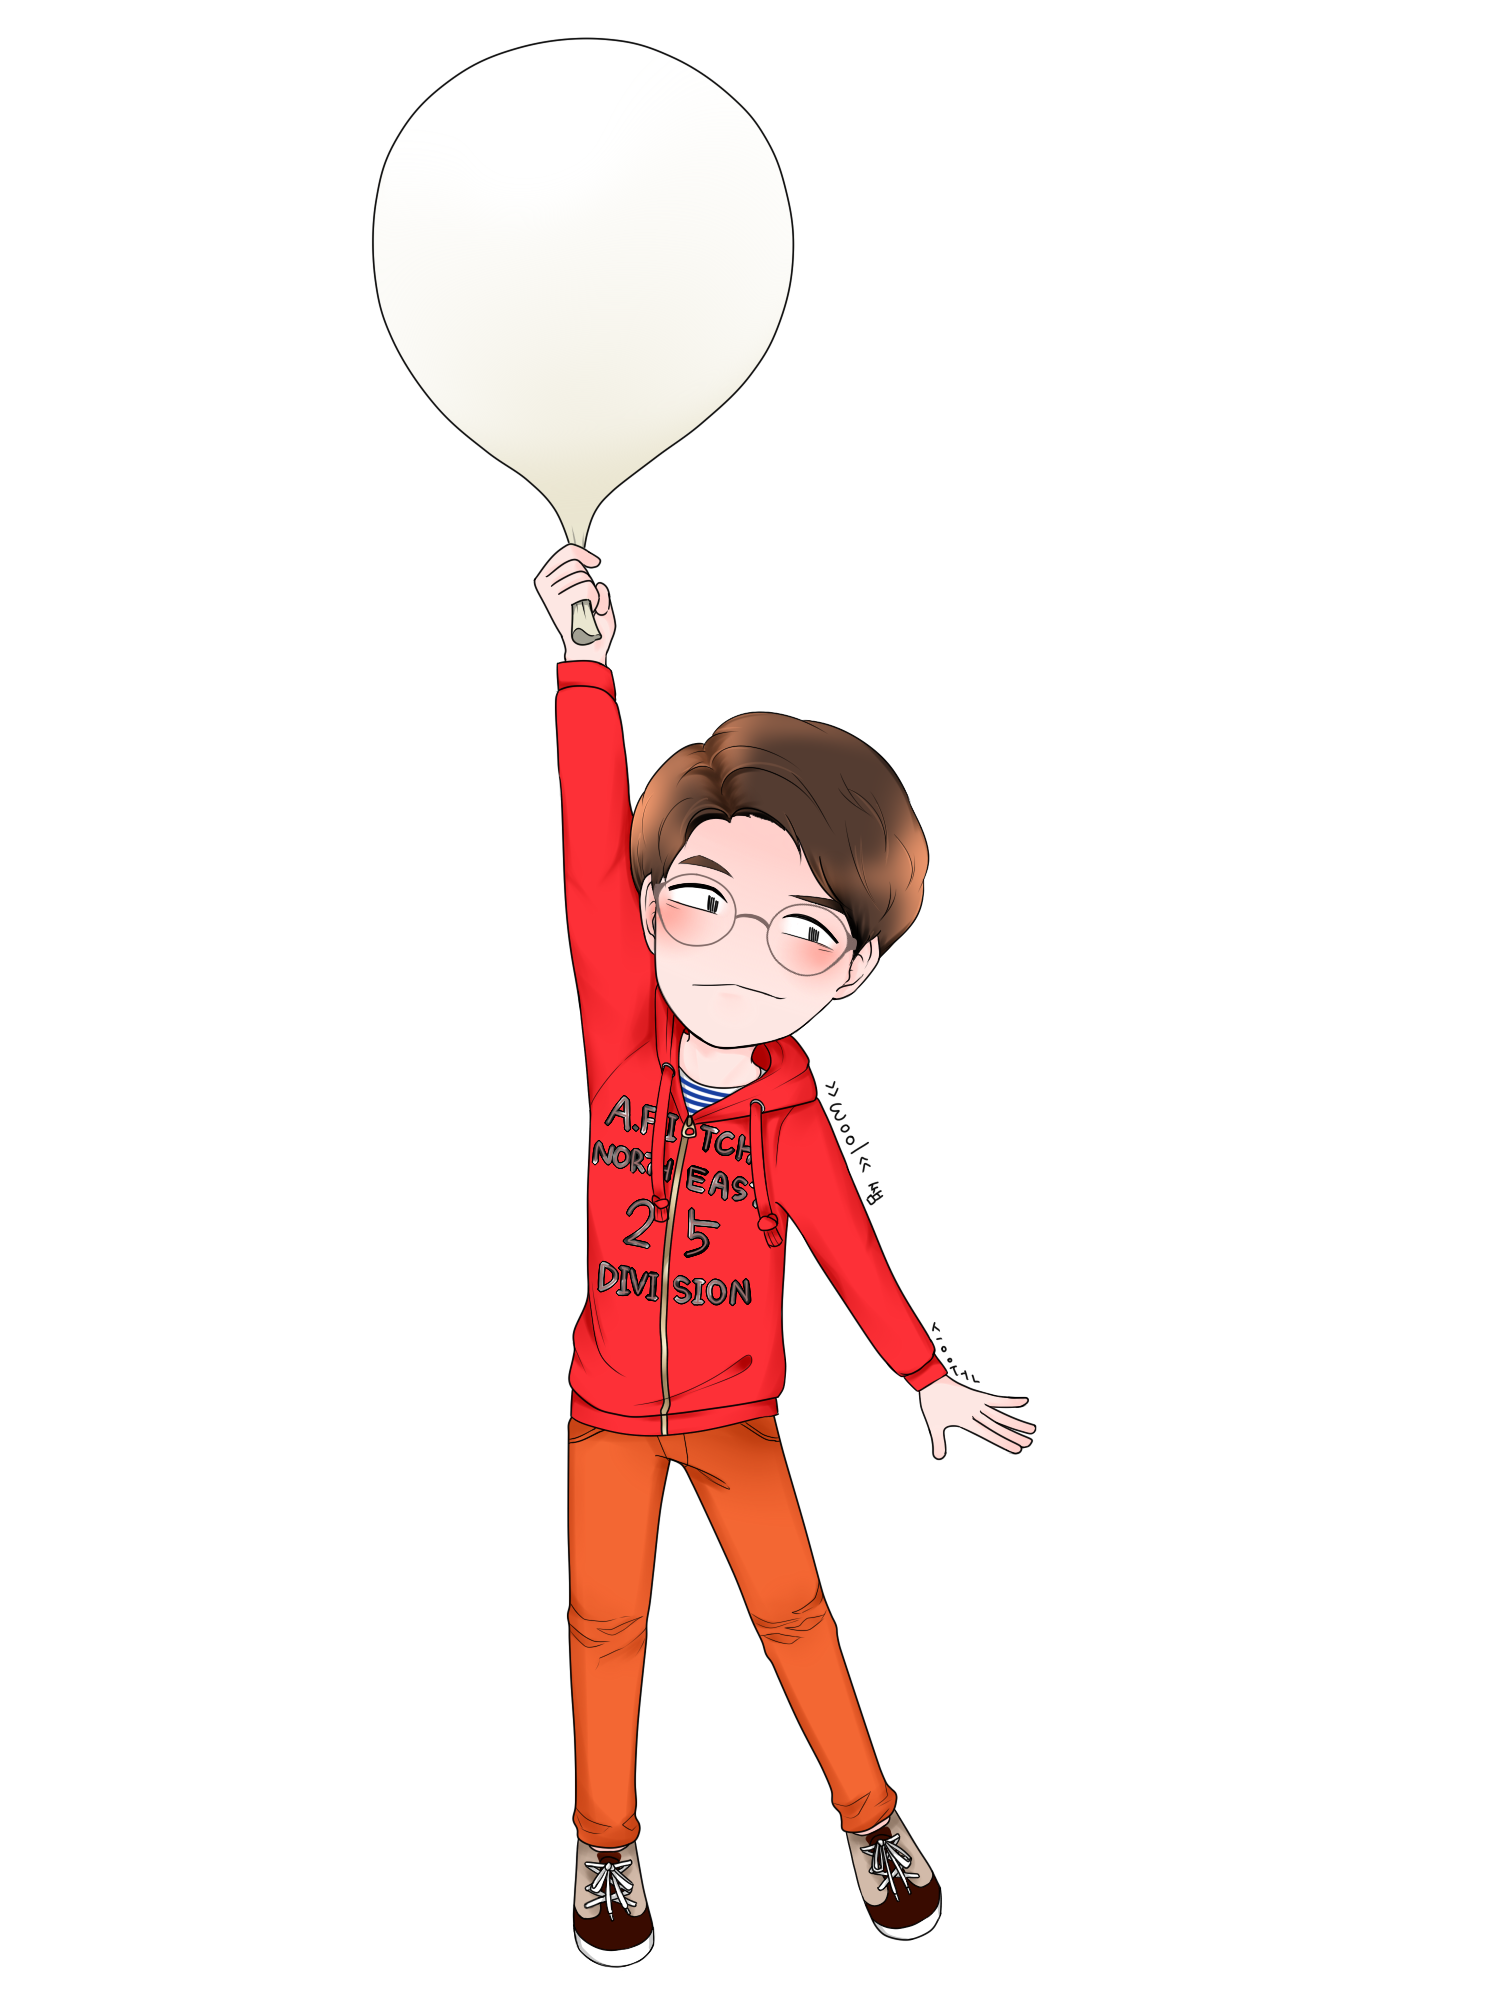
\includegraphics[width=0.4\paperwidth]{./logo/100_01.png}%
      
\includegraphics[width=0.7\paperwidth]{./logo/gshslogo2.jpg}%
    \end{picture}%
    }%
  \end{picture}%
  \vfill
  \vspace*{10mm}
  \raggedleft
  %% Title
  \usebeamerfont{title}\usebeamercolor[fg]{title}\inserttitle\par
  \vskip 2mm
  %% Subtitle
  \ifx\insertsubtitle\@empty
  \else\usebeamerfont{subtitle}\usebeamercolor[fg]{subtitle}\insertsubtitle
  \fi

  \vskip 3mm
  %% Horizontal line
  \usebeamercolor[fg]{title}\hrule height 2pt\hfill
  \vskip 10mm
  %% Author
  \usebeamercolor[fg]{author}\usebeamerfont{author}\insertauthor
  \vskip 1cm
  %% Institute
  \usebeamercolor[fg]{institute}\usebeamerfont{institute}\insertinstitute
  \vskip 1cm
  %% Date
  %\usebeamercolor[fg]{date}\usebeamerfont{date}\insertdate
  \vfill
}

%% itemize bullet setting %%
\setbeamertemplate{itemize items}[ball]

%% block setting %%
\setbeamertemplate{blocks}[rounded][shadow=true]

%% Title, Author, Institute, Date %%
\title[]{정육면체의 정사영의 넓이의 최댓값 \\: 엄밀한 접근}
\subtitle[]{수학세미나 I}
\author[]{15011 김경태}
\institute[GSHS]{경기과학고등학교}
\date[]{\today}

%%%%%%%%%%%%%%%%%%%%%%%%%%%%%%%%%%%%%%%%%
%\logo{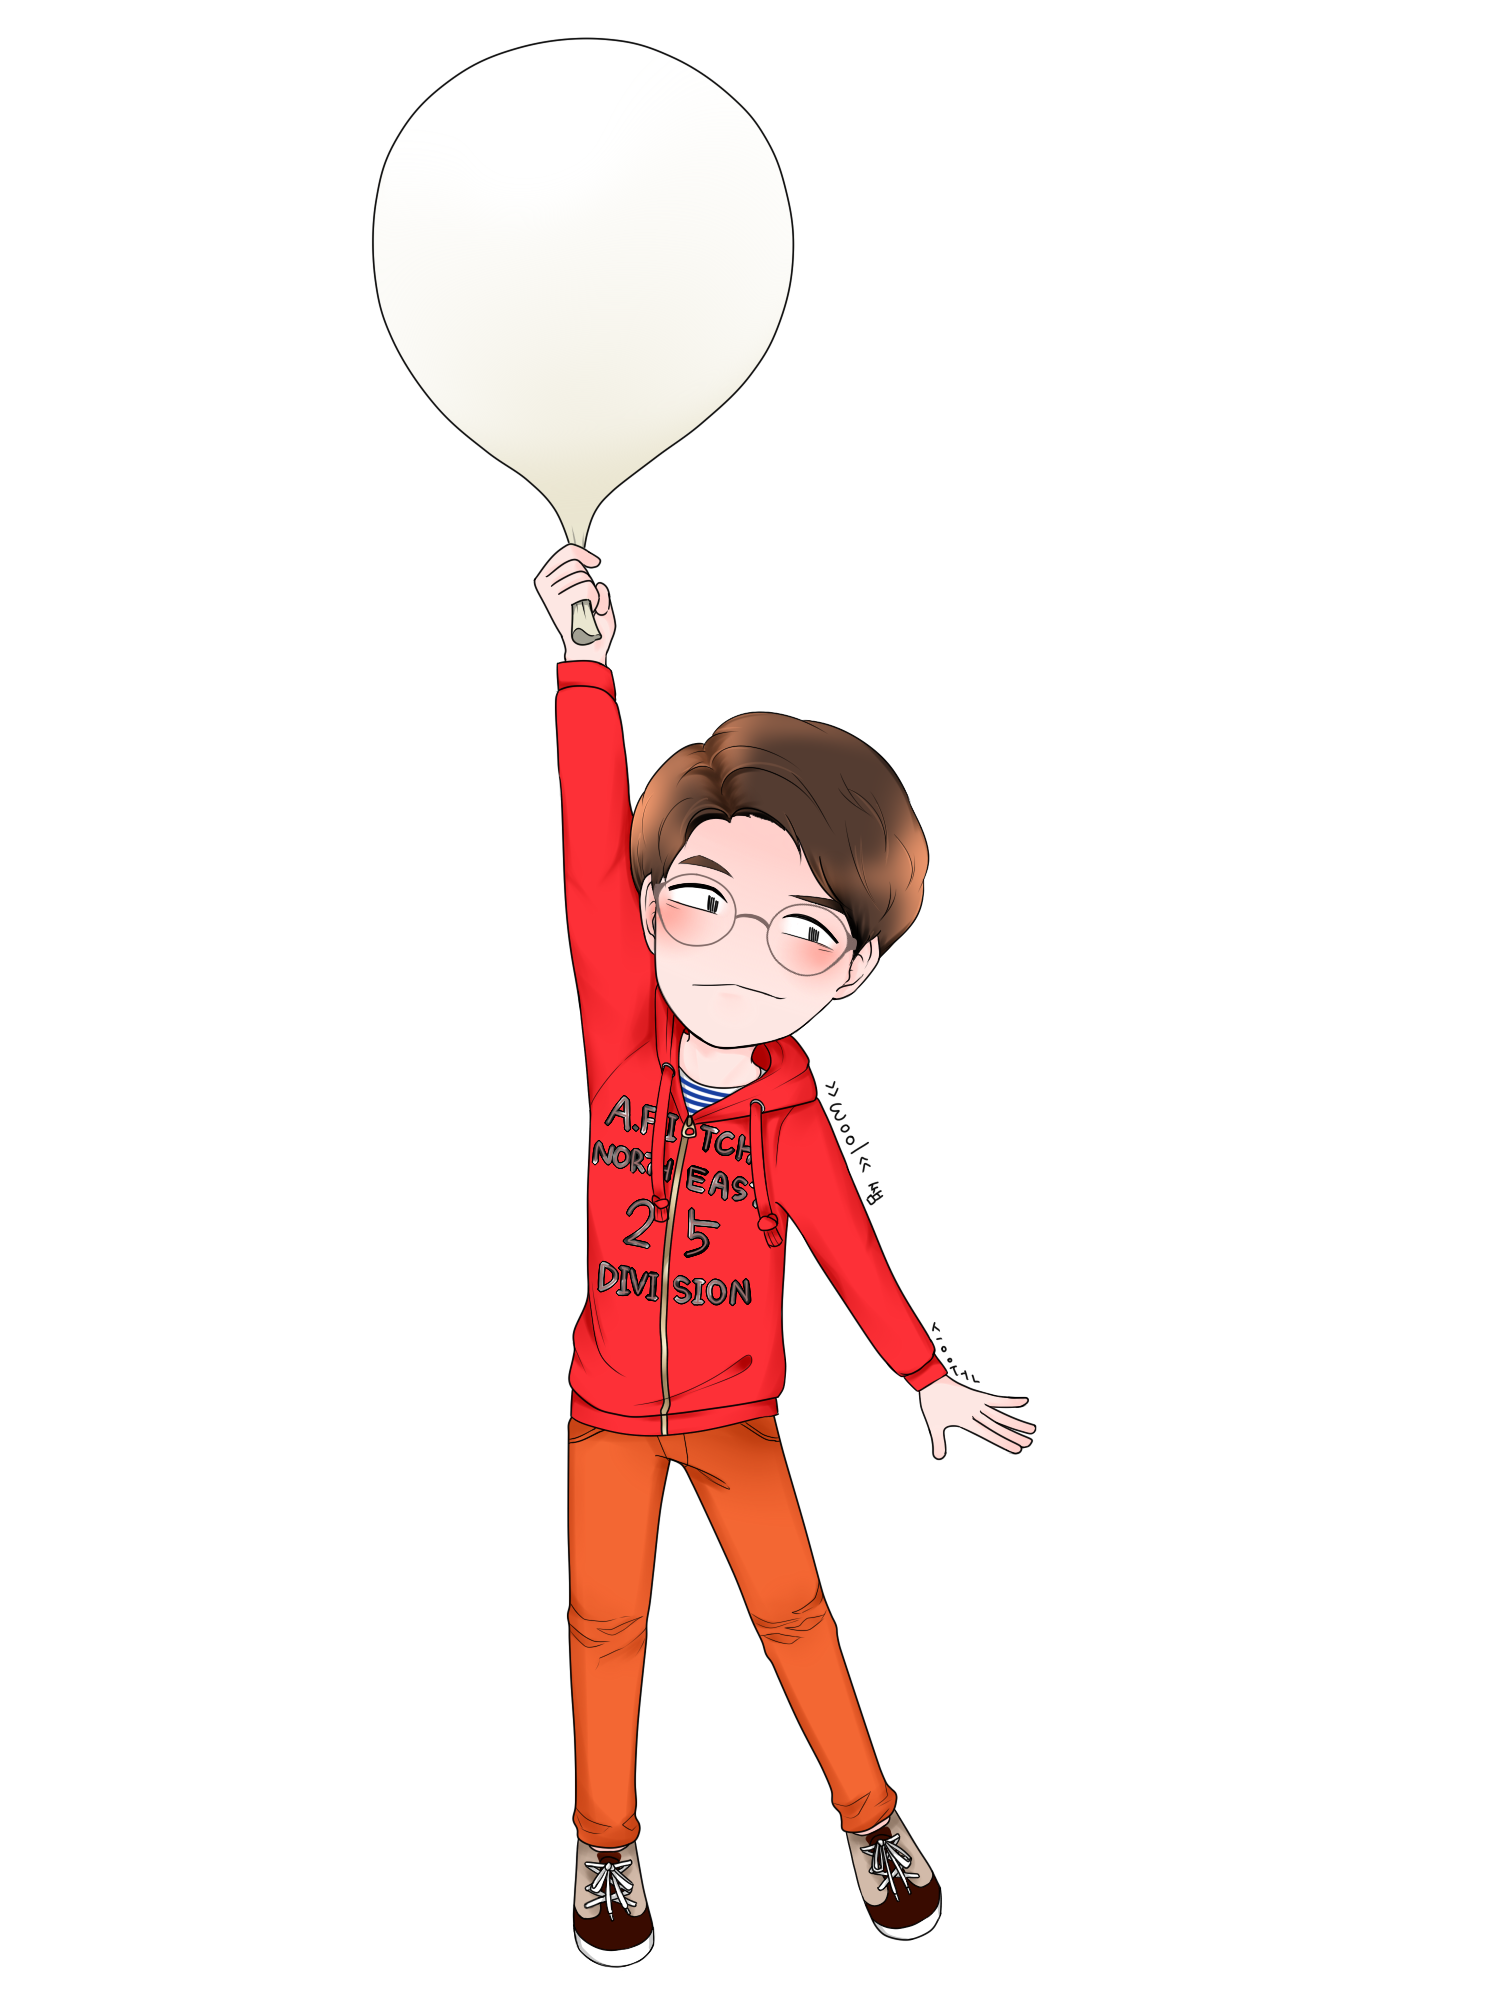
\includegraphics[width=15mm]{./logo/100_01.png}}
\logo{
\includegraphics[width=8mm]{./logo/gshslogo.png}}

%% Main %%
\begin{document}

\begin{frame}[plain]
\titlepage
\end{frame}
\setbeamertemplate{sidebar left}[sidebar theme]

\setstretch{1.1} %줄간격


\section{Problem Statement}

\subsection{Problem}
\begin{frame}
	\begin{block}{문제}
		한 변의 길이가 1인 정육면체가 있다. 이 정육면체가 평면 위에 정사영될 때, 정사영된 정육면체의 넓이의 최댓값을 구하여라.
	\end{block}
	(풀이) 정육면체를 정사영시킬 때 최대 세 면이 (유효하게) 정사영된다 (Why?). 그 중 세 면이 정사영될 때 넓이가 최대가 되고, 세 면이 정사영할 평면과 이루는 각을 각각 $\theta_1, \theta_2, \theta_3$이라 하면, 
	\[\cos^2\theta_1 + \cos^2\theta_2 +\cos^2\theta_3=1\]
	이고 정사영의 넓이는 
	\[S=\cos\theta_1+\cos\theta_2+\cos\theta_3\]
	이다 (Why? 두 면의 정사영이 겹친다면?). 코시-슈바르츠 부등식을 이용하여 $S$의 최댓값을 구할 수 있다.
\end{frame}

\subsection{Definition}
\begin{frame}
	정사영될 평면을 $z=0$이라 하자. 정육면체의 8개 꼭짓점 중 $z$ 좌표가 가장 작은 꼭짓점이 원점에 오도록 정육면체를 평행이동하자. 그 다음에 원점과 모서리로 연결된 세 꼭짓점의 위치벡터를 $\mathbf{w}_1, \mathbf{w}_2, \mathbf{w}_3$라 하자. 
	
	공간 상의 한 점을 그 점의 정사영으로 보내는 변환은 선형변환이다. $z=0$으로의 정사영을 나타내는 선형변환을 $T: \mathbb{R}^3 \to \mathbb{R}^2$이라 하자. 정육면체의 내부와 경계를 집합 $G$라 하고 $R=T(G)$라 하자. 또한 정육면체 중에서 원점을 공유하는 세 면을 집합 $G'$라 하고 $R'=T(G')$라 하자. 우리의 목표는 $R=R'$임을 보이는 것이다.
\end{frame}

\begin{frame}
	앞의 정의에 의하여,
	\begin{align*}
	G&=\{c_1 \mathbf{w}_1 + c_2 \mathbf{w}_2 + c_3 \mathbf{w}_3|0 \leq c_1, c_2, c_3 \leq 1\},\\
	R&=\{c_1 T(\mathbf{w}_1) + c_2 T(\mathbf{w}_2) + c_3 T(\mathbf{w}_3)|0 \leq c_1, c_2, c_3 \leq 1\},\\
	G'&=\cup_{i<j} \{a \mathbf{w}_i + b \mathbf{w}_j|0 \leq a,b \leq 1\},\\
	R'&=\cup_{i<j} \{a T(\mathbf{w}_i) + b T(\mathbf{w}_j)|0 \leq a,b \leq 1\}.
	\end{align*}
	우리는 정육면체가 평면에 원점에서만 닿는 경우만 고려하자. 나머지 경우(모서리가 닿거나 면이 닿는 경우)는 이것보다 훨씬 간단하다.
\end{frame}

\section{Solution}
\begin{frame}
	\begin{block}{Proposition 1}
		$T(\mathbf{w}_1), T(\mathbf{w}_2), T(\mathbf{w}_3)$는 서로 둔각을 이룬다.
	\end{block}
(증명) $\mathbf{w}_1=(x_1, y_1, z_1), \mathbf{w}_2=(x_2, y_2, z_2)$라 하자. $\mathbf{w}_1 \cdot \mathbf{w}_2=x_1x_2 + y_1y_2 + z_1z_2=0$이고 $z_1, z_2>0$인데,
\begin{align*}
T(\mathbf{w}_1) \cdot T(\mathbf{w}_2)&=(x_1,y_1,0) \cdot (x_2,y_2,0) \\
&= x_1y_1+x_2y_2 \\
&< x_1y_1+x_2y_2+x_3y_3=0 
\end{align*}
이므로 $T(\mathbf{w}_1)$과 $T(\mathbf{w}_2)$는 둔각을 이룬다.
	
\end{frame}

\begin{frame}
	\begin{block}{Proposition 2}
		$T(\mathbf{w}_1), T(\mathbf{w}_2), T(\mathbf{w}_3)$ 중 어느 두 개도 linearly independent하다.
	\end{block}
(증명) $T(\mathbf{w}_1), T(\mathbf{w}_2)$가 linearly dependent하다고 가정하면, 스칼라 $c$가 존재하여 $T(\mathbf{w}_1)+ cT(\mathbf{w}_2)=\mathbf{0}$이다. 즉 $W$를 $z=0$인 평면을 나타내는 $\mathbb{R}^3$의 subspace라 하면 $\mathbf{w}_1+c\mathbf{w}_2 \in W^\perp$이다. $\mathbf{w}_1+c\mathbf{w}_2 \neq \mathbf{0}$이고 $\rm{dim} W^\perp=1$이기 때문에 $\{\mathbf{w}_1+c\mathbf{w}_2\}$는 $W^\perp$의 basis인데, $\mathbf{w}_3 \cdot (\mathbf{w}_1+c\mathbf{w}_2)=0$이므로 $\mathbf{w}_3 \in (W^\perp)^\perp=W$가 된다. 즉 $\mathbf{w}_3$이 정사영할 평면 위에 있어, 정육면체의 한 점만 평면과 닿아있다는 가정에 모순이다.
\end{frame}

\begin{frame}
	\begin{block}{Proposition 3}
		스칼라 $c_1,c_2$에 대하여 $T(\mathbf{w}_3)=c_1 T(\mathbf{w}_1) + c_2T(\mathbf{w}_2)$로 나타낼 때 $c_1,c_2<0$이다.
	\end{block}
(증명) 자명.
\end{frame}

\begin{frame}
	\begin{block}{Theorem 4}
		$G'$을 이루는 세 면 중 임의의 서로 다른 두 면의 정사영의 intersection은 선분이고, 그 넓이는 0이다.
	\end{block}
(증명) $\mathbf{w}_1, \mathbf{w}_2$로 만들어지는 면과 $\mathbf{w}_2, \mathbf{w}_3$으로 만들어지는 두 면을 고려하자.  두 영역의 점이 변환 $T$ 이후에 같으려면 스칼라 $a,b,c,d \in[0,1]$에 대하여
\[aT(\mathbf{w}_1)+bT(\mathbf{w}_2)=cT(\mathbf{w}_2)+dT(\mathbf{w}_3)\]
또는
\[aT(\mathbf{w}_1)+(b-c)T(\mathbf{w}_2)-dT(\mathbf{w}_3)=\mathbf{0}\] 
이면 된다. $b>c$이면 $T(\mathbf{w}_3)$은 $T(\mathbf{w}_1)$과 $T(\mathbf{w}_2)$에 음수를 곱한 선형결합으로 나타내어지기 때문에 위 식이 성립할 수가 없다. $b<c$인 경우에는 $T(\mathbf{w}_1)$에 대해 같은 논리를 적용하면 마찬가지가 된다. 남은 경우인 $b=c, a=d=0$일 때만 위 식이 성립하고, 그에 해당하는 영역이 바로 원점과 $T(\mathbf{w}_2)$를 잇는 선분이다.
\end{frame}

\begin{frame}
	\begin{block}{Theorem 5}
		$R=R'$이다. 즉, 정육면체의 세 면의 정사영만 고려해도, 정육면체의 나머지 부분이 세 면의 정사영 안에 들어오기 때문에 충분하다.
	\end{block}
(증명) $\mathbf{v}_i=T(\mathbf{w}_i)$로 표기하자. 다음과 같이 세 집합으로 $\mathbb{R}^2$를 분할하면,
\begin{align*}
S_1&=\{c_2 \mathbf{v}_2+c_3\mathbf{v}_3|c_2,c_3 \geq 0\},\\
S_2&=\{c_3 \mathbf{v}_3+c_1\mathbf{v}_1|c_3,c_1 \geq 0\},\\
S_3&=\{c_1 \mathbf{v}_1+c_2\mathbf{v}_2|c_1,c_2 \geq 0\}.
\end{align*}
 일반성을 잃지 않고 $\mathbf{v}=c_1\mathbf{v}_1+c_2\mathbf{v}_2+c_3\mathbf{v}_3 \in S_3$이라 하자. $a,b<0$에 대하여 $\mathbf{v}_3=a \mathbf{v}_1 + b\mathbf{v}_2$이므로, 
\[ \mathbf{v}=(c_1+ac_3)\mathbf{v}_1 + (c_2+bc_3)\mathbf{v}_2\]
이고 $0 \leq c_1+ac_3, c_2+bc_3 \leq 1$이므로 $\mathbf{v} \in R'$이다.
\end{frame}


\end{document}